%/*% pdflatex -file-line-error -interaction nonstopmode %

\documentclass{article}
\usepackage{graphicx}
\usepackage{amsmath}
\usepackage{amsfonts}
\usepackage{bookmark}
\usepackage{booktabs}
\usepackage{exercises}
\graphicspath{ {./images/3.5} }
\usepackage{indentfirst}
\usepackage{amsthm}
\usepackage{yhmath}
\usepackage{placeins}
\newcommand*{\oldneg}{\mathord{\sim}}
\newcommand\showdiv[1]{\overline{\smash{)}#1}}
\newcommand\Mydiv[1]{%
\smash{\raise.3ex\hbox{$\big)$}}\mkern-8mu
        \overline{\enspace\strut#1}}
\setlength{\tabcolsep}{5pt}
\theoremstyle{definition}
\newtheorem{definition}{Definition}

\setlength{\parindent}{.5in}
\setlength{\parskip}{12pt}
\renewcommand{\arraystretch}{2}

\title{3.5 Answers}
\begin{document}
\maketitle

\section*{1}
Square root functions and cube root functions are examples of radical functions.

\section*{2}
(a): If $a=-3$, the graph will be reflected over the $x$-axis (to be negative) and will expand by a factor of 3.\newline
(b): If $h=2$, then the graph will be shifted to the right by 2 units.\newline
(c): If $k=4$, then the graph will be shifted up by 4 units.

\section*{7}
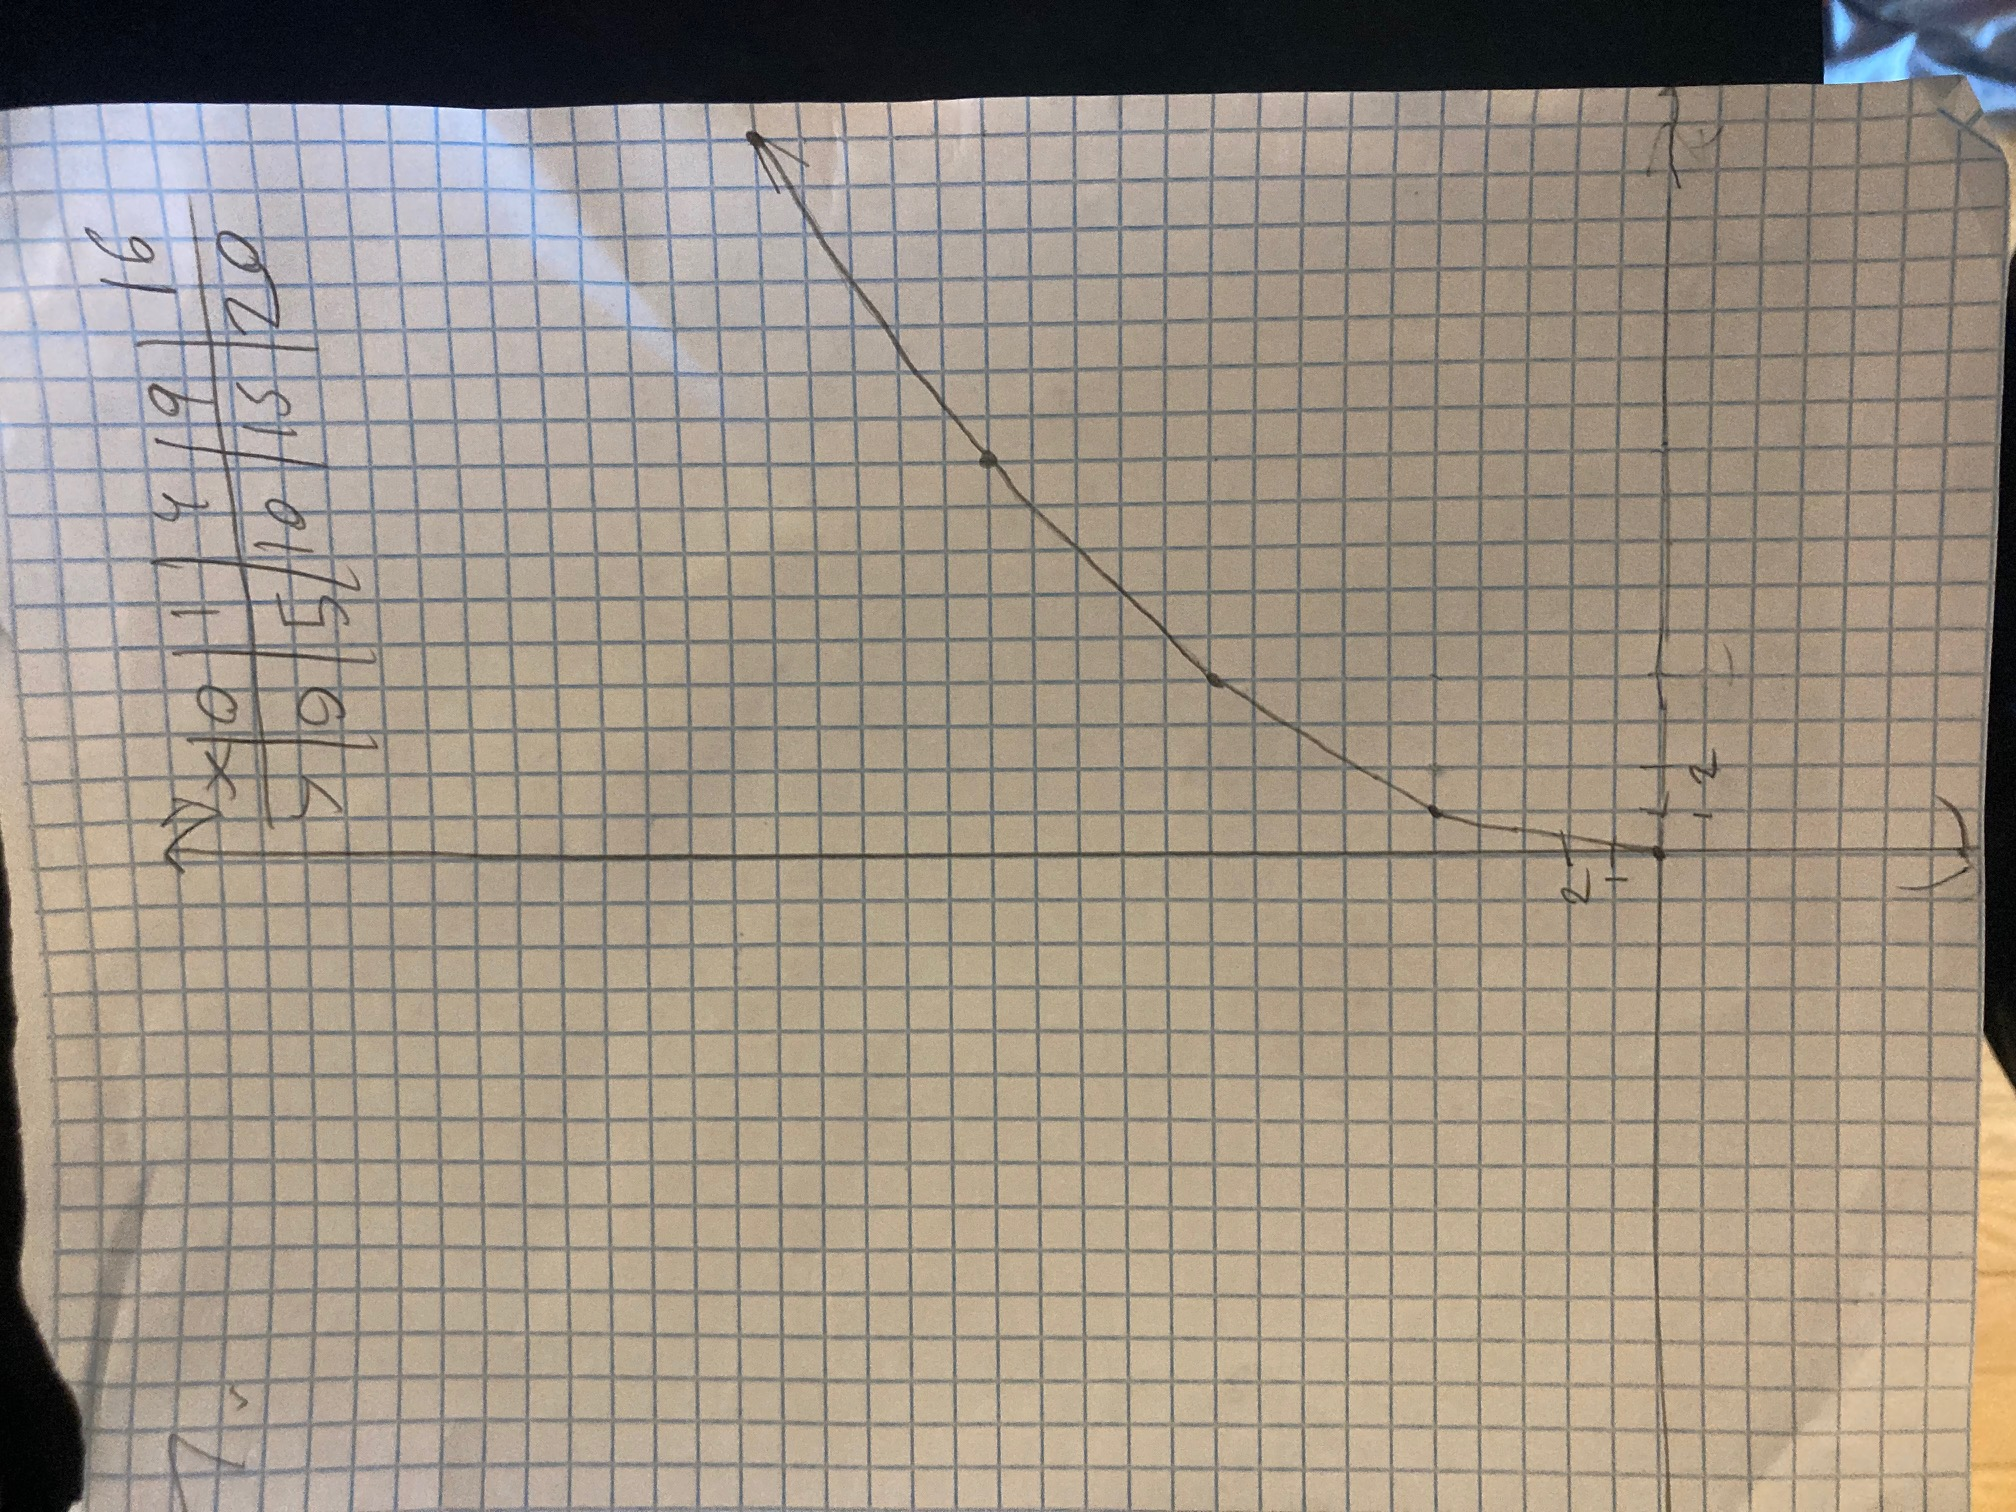
\includegraphics[width = 4in, height = 4in, angle=-90]{picture7}
\newline The domain of the function is $x\ge 0$, as we cannot take negative square roots. This means that the range of the function is 
$\ge \sqrt{5}(0)=0$.

\section*{9}
D

\section*{20}
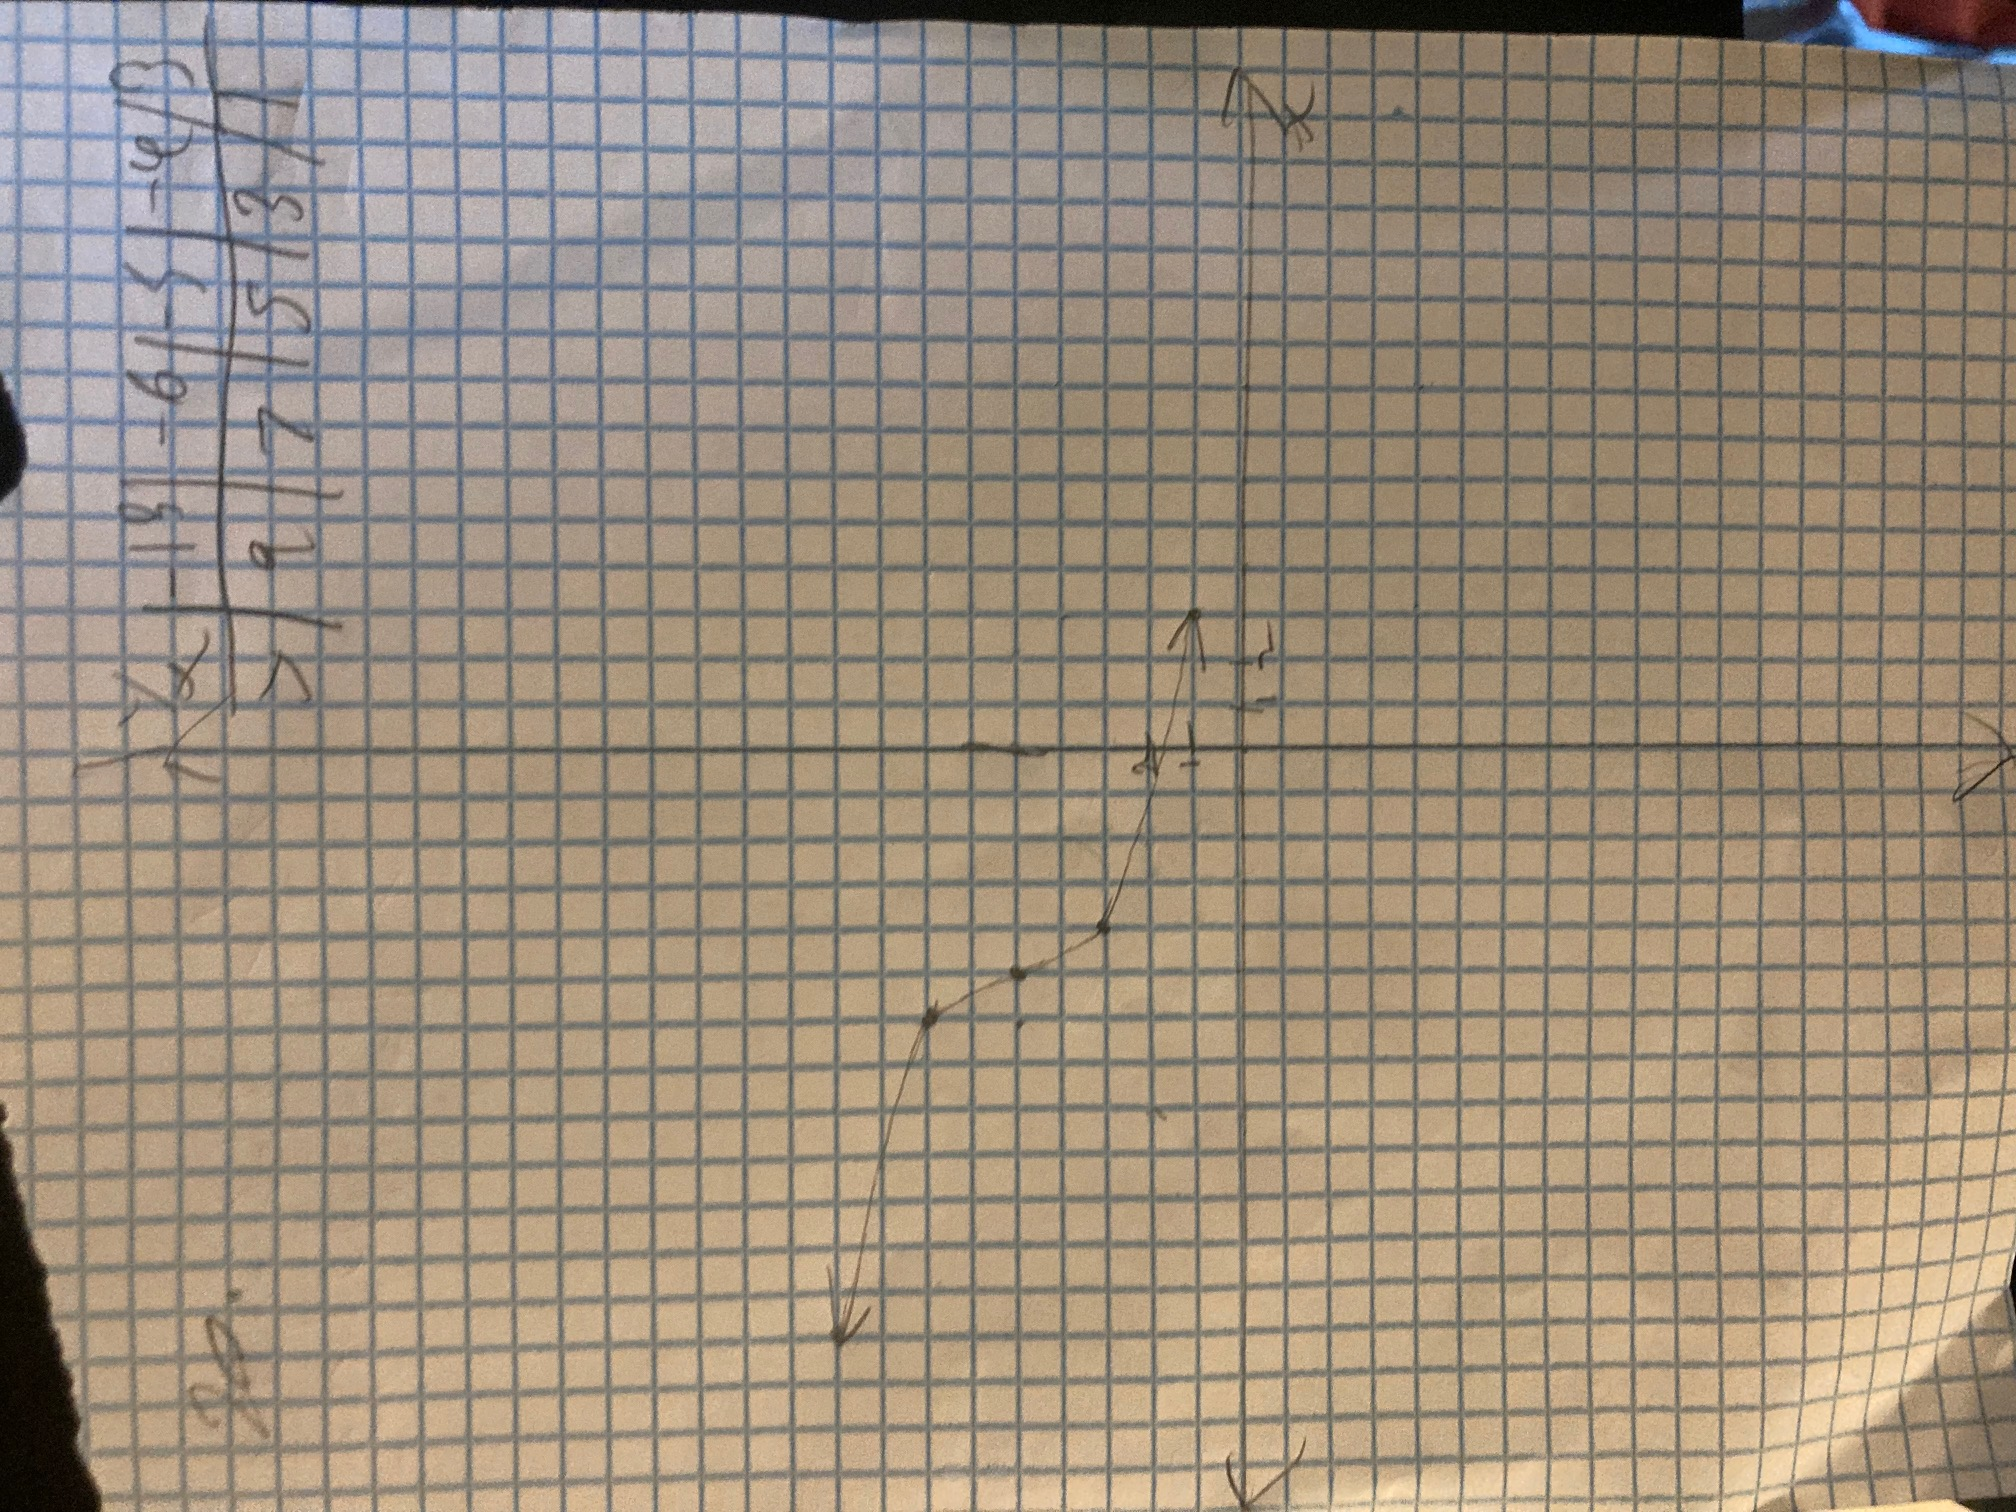
\includegraphics[width = 4in, height = 4in, angle=-90]{picture20}
\newline Both the domain and the range of the function are all real numbers. 

\section*{22}
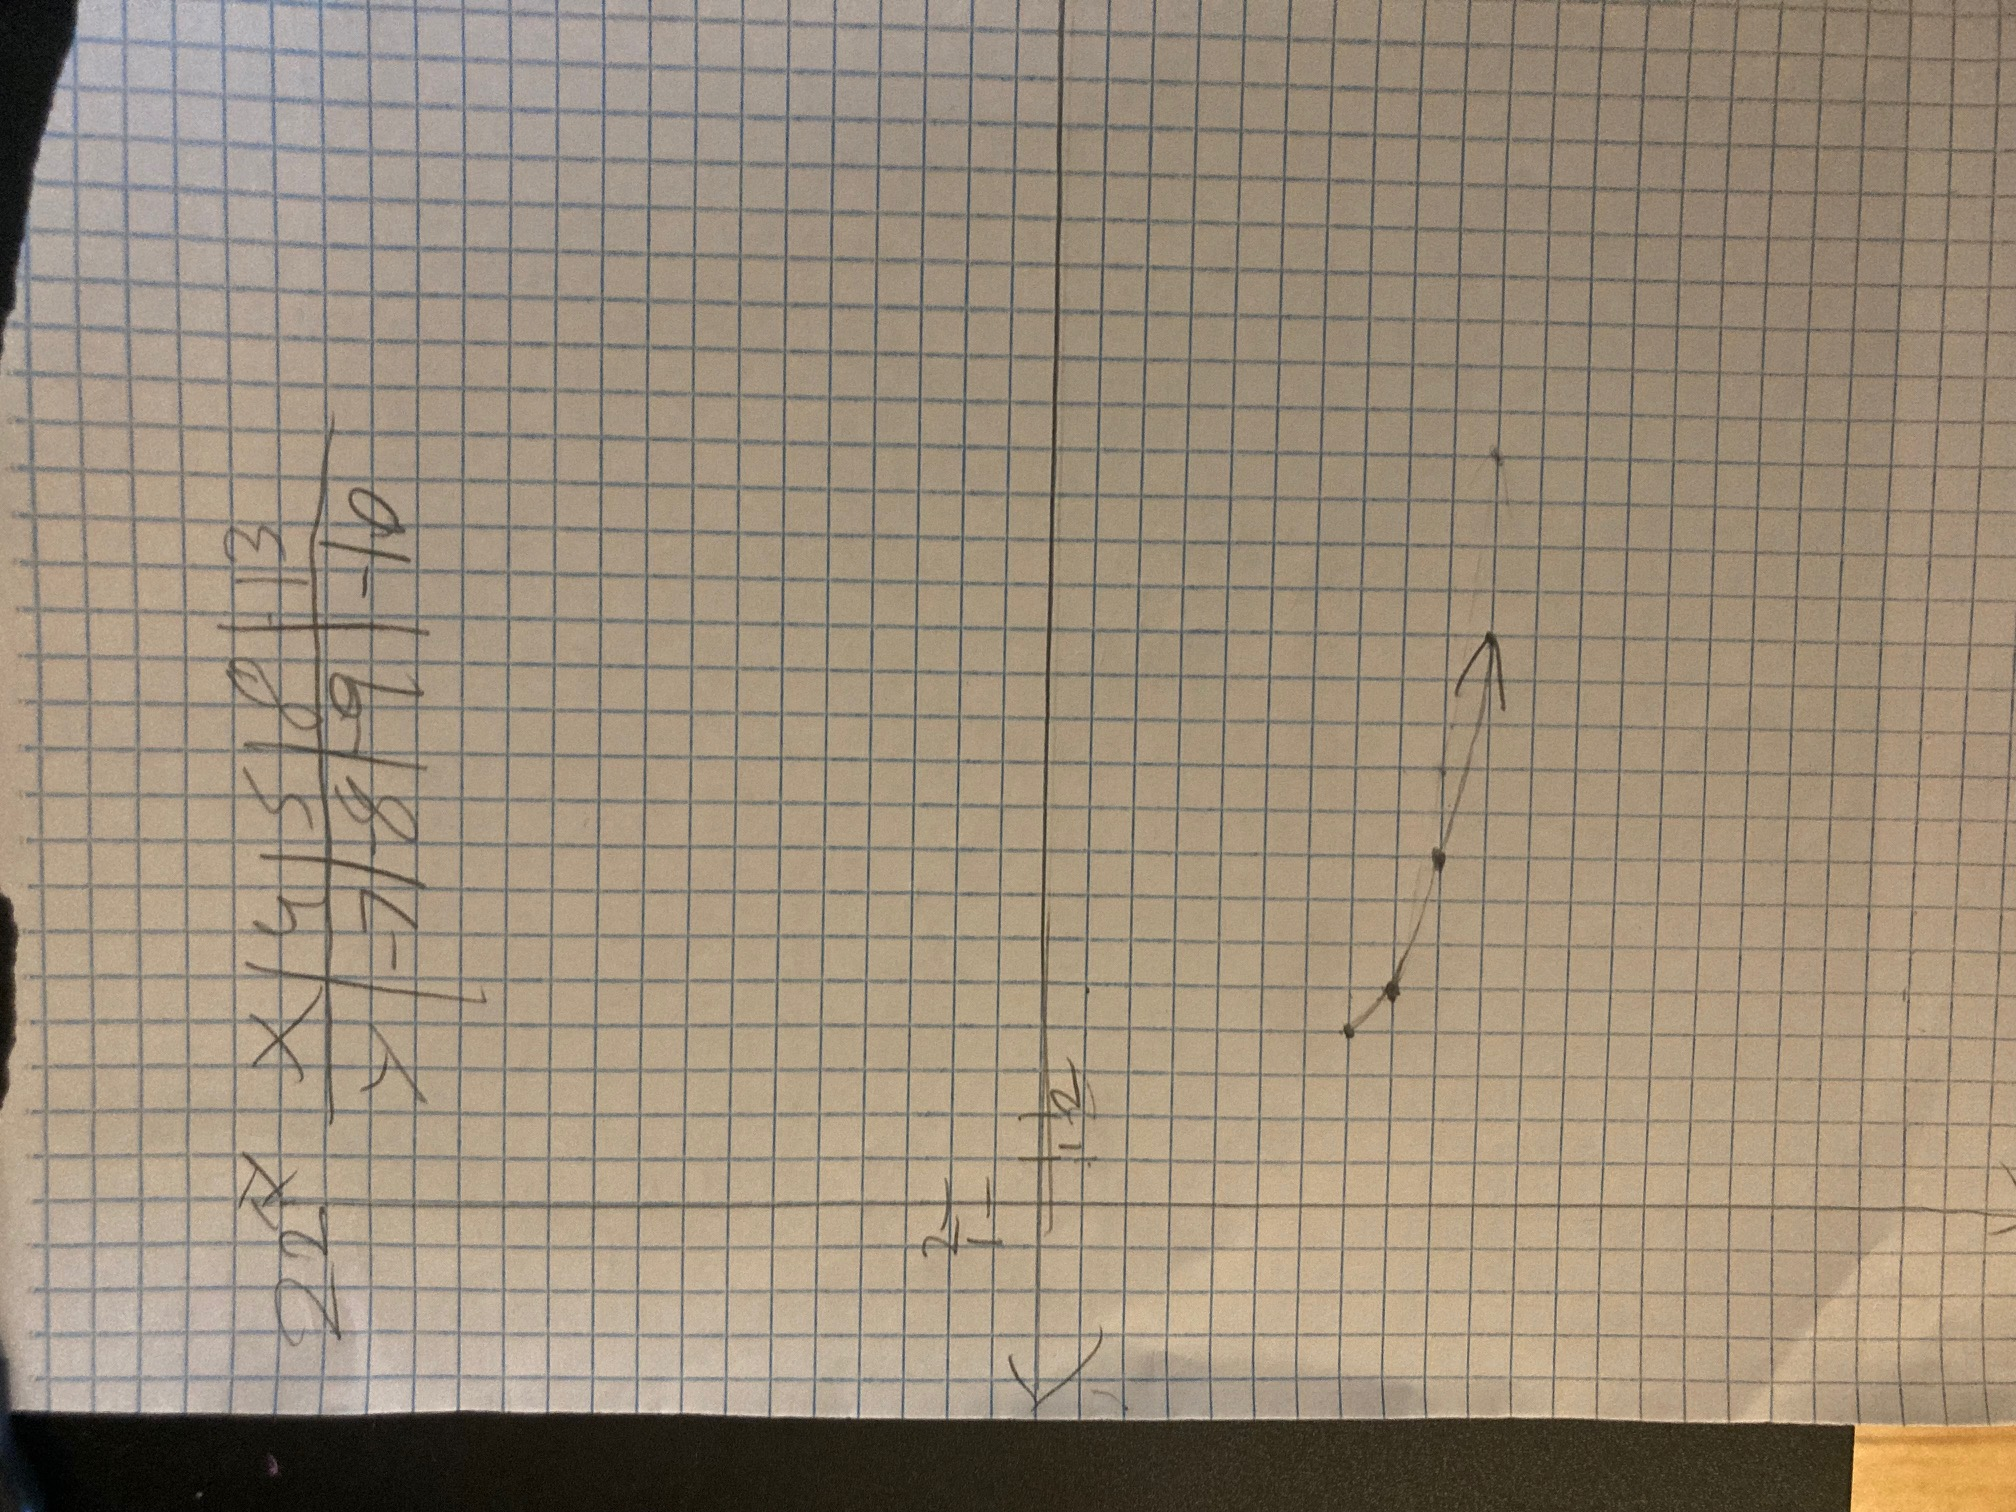
\includegraphics[width = 4in, height = 4in, angle=-90]{picture22}
\newline The domain of the function is $x\ ge 4$, as $x<4$ would mean $\sqrt{x-4}$ would take a square root of a negative number. Because 
$x\ge 4$, the range of the function is $y\le -\sqrt{4-4}-7=-7$.


\section*{25}
There are limitations on the domain, as any $x$ value $<5$ will be taking the square root of a negative number, which is impossible. Thus 
$x\ge 5$. Also, because $\sqrt{x-5}\ge 0$, $\sqrt{x-5}+4\ge 4$, meaning $y\ge 4$. 

\section*{26}
The error here is that the student forgot that the $h$ units the graph will shift by is given from the equation 
$y=a\sqrt[3]{x-h}+k$, not $y=a\sqrt[3]{x+h}+k$, meaning a value of $h=-1$ actually shifts the graph to the left one unit. Thus, the graph shifts to the 
left one unit, and down 3 units.

\section*{27} 
C

\section*{33}
The domain of the function is $x\ge 3$, as $x<3$ would imply $\sqrt{x-3}$ takes the square root of a negative number, which is impossible. Also, 
because $\sqrt{x-3}\ge 0$, $\frac{1}{4}\sqrt{x-3}+6\ge 6$, meaning $y\ge 6$.

\section*{37}
(a): We are given that $K=273.15+C$. We are to write an equation that gives $v$ as a function of $C$, the temperature in celsius. If 
we let $f(C)=273.15+C$, and $g(K)=331.5\sqrt{\frac{K}{273.15}},K\ge 0$, the desired function is just $g(f(C))$, which is:
\[ 331.5\sqrt{\frac{273.15+C}{273.15}},C\ge 273.15 \]
(b): A reasonable domain is $C\ge 273.15$, as this is just the given domain of the function. Because $\sqrt{\frac{273.15+C}{273.15}}$ cannot be 
negative, a reasonable range of the function is $y\ge 0$.

\section*{40}
(a): \[ S=\pi r+\pi r^2 \] \[ S=\pi(r+r^2) \] \[ S+\frac{\pi}{4}=\pi(r^2+r+\frac{1}{4}) \] \[ S+\frac{\pi}{4}=\pi(r+\frac{1}{2})^2 \]
\[ \frac{1}{\pi}(S+\frac{\pi}{4})=(r+\frac{1}{2})^2 \] \[ \frac{1}{\sqrt{\pi}}\sqrt{S+\frac{\pi}{4}}=r+\frac{1}{2} \]
\[ \frac{1}{\sqrt{\pi}}\sqrt{S+\frac{\pi}{4}}-\frac{1}{2}=r \]
(b): \newline 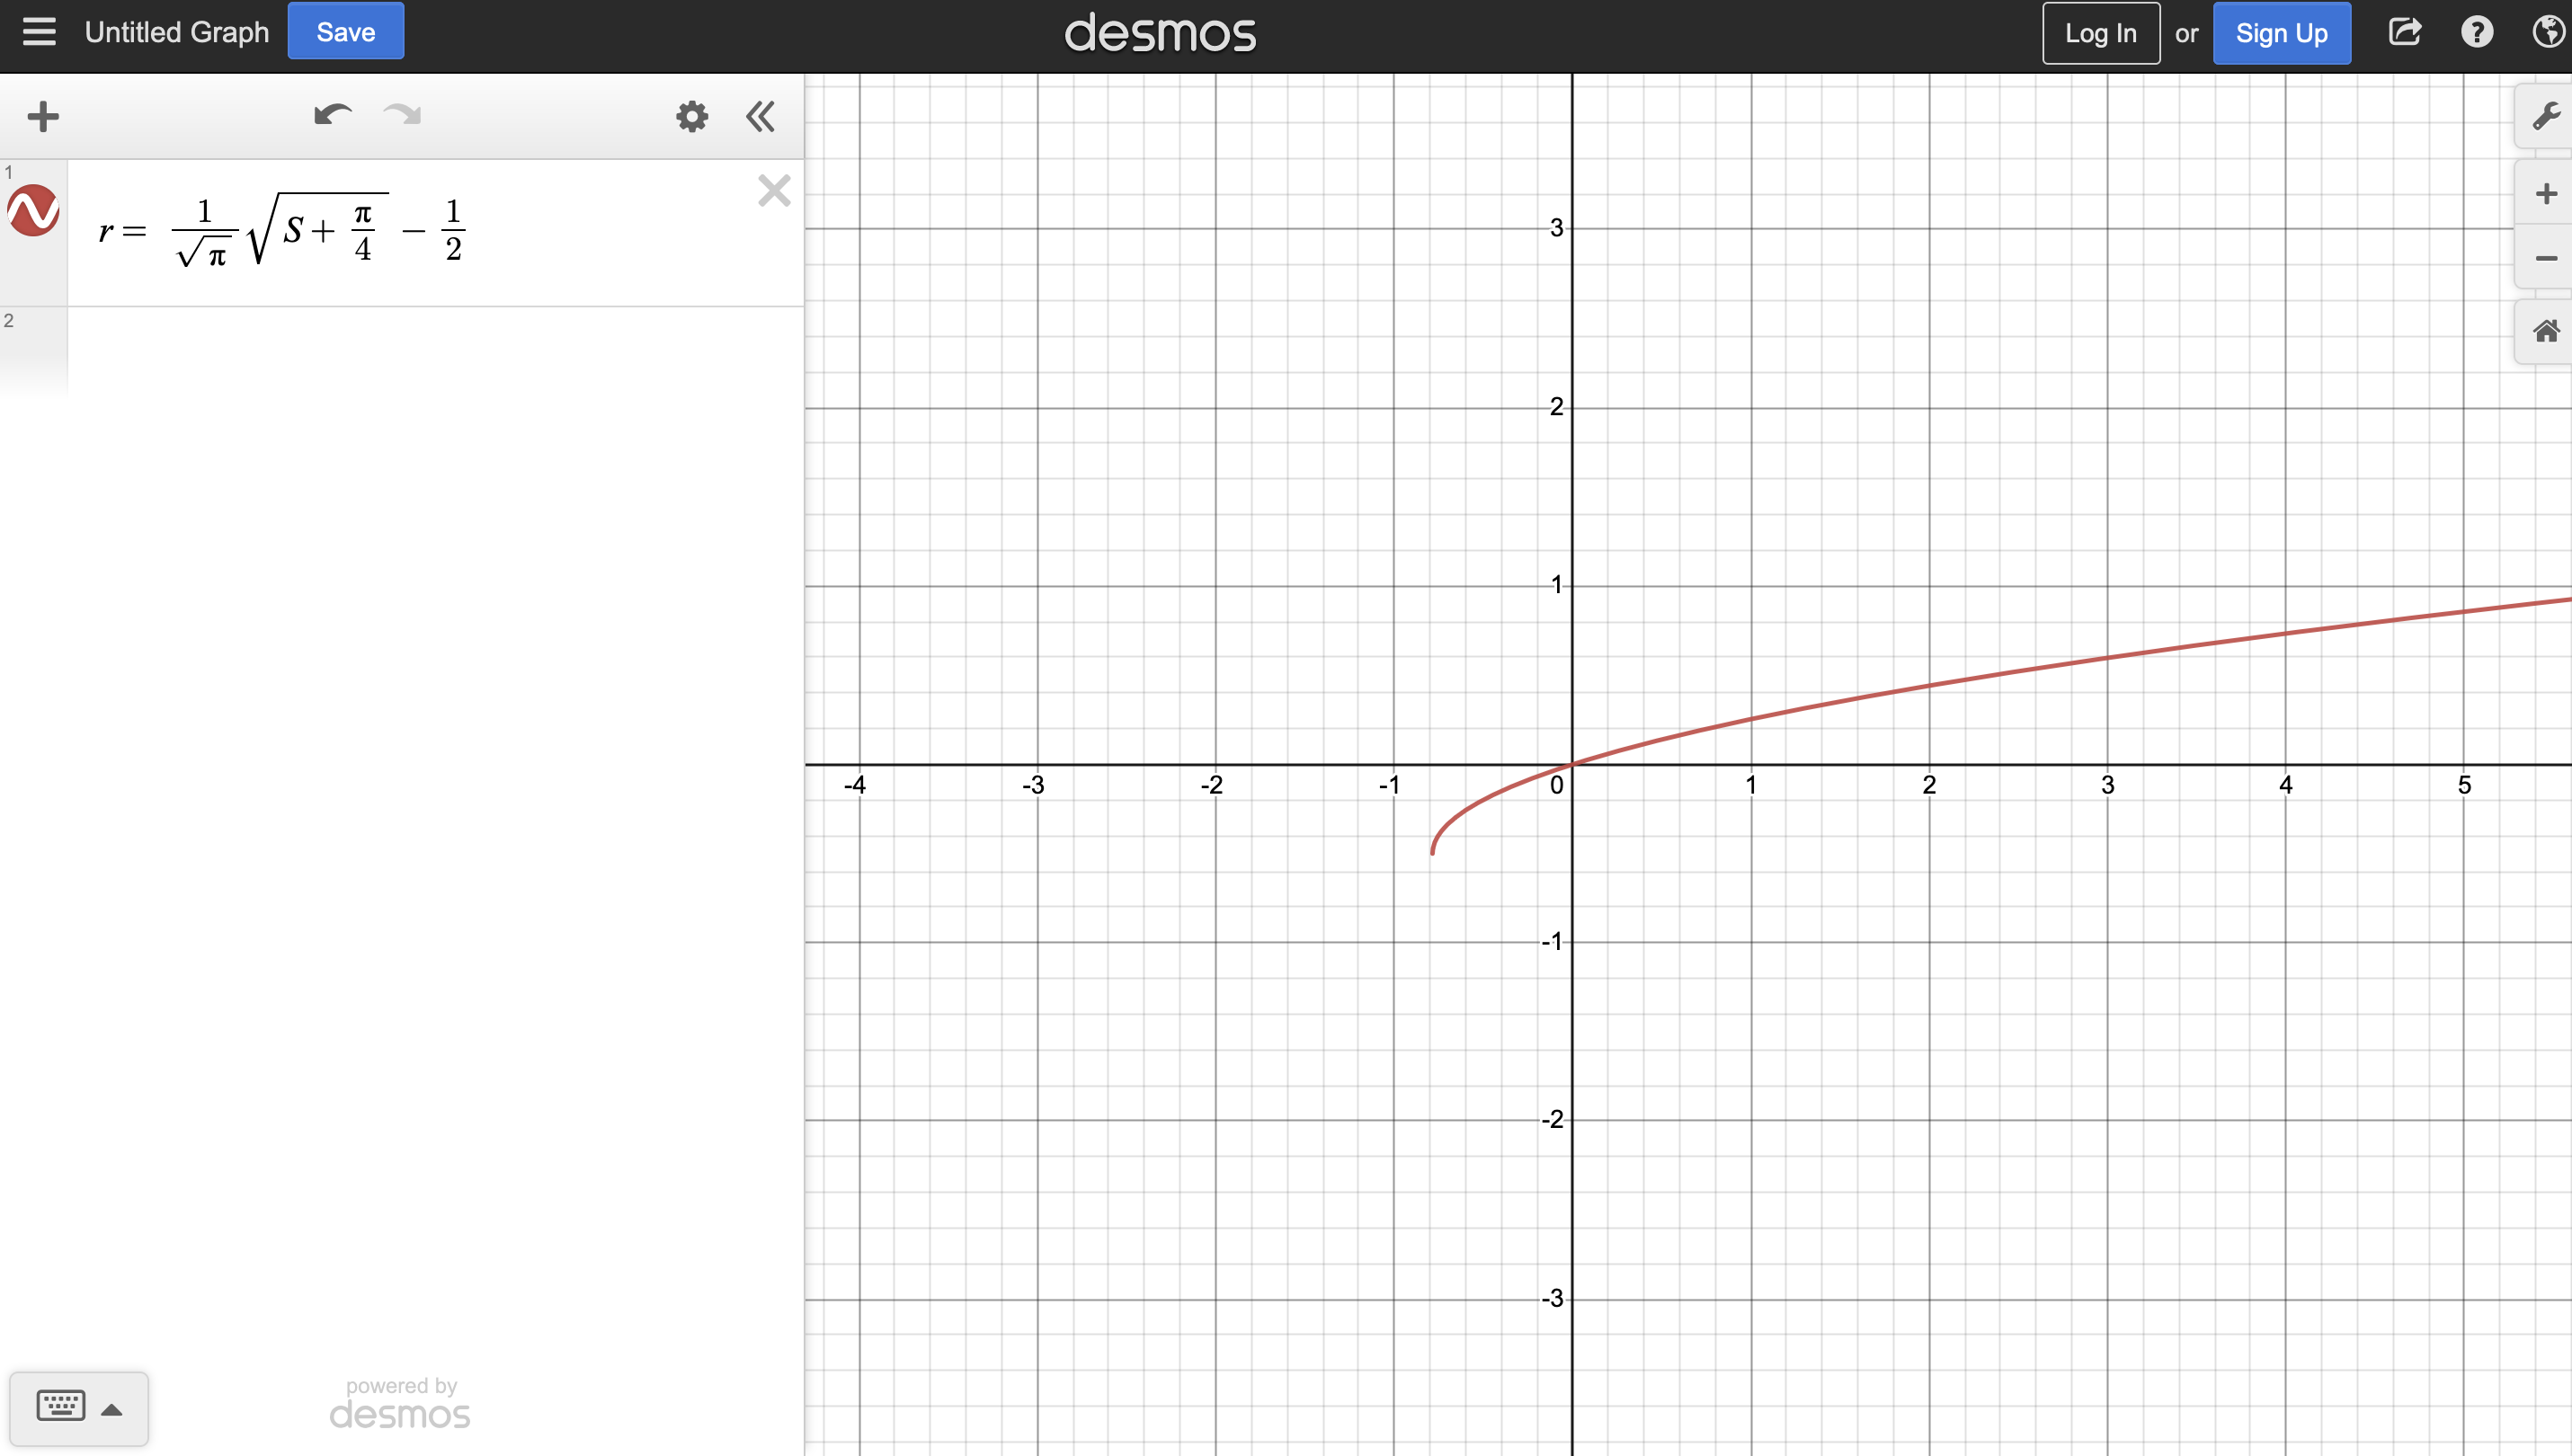
\includegraphics[width = 4in, height = 4in]{picture40}\newline
(c): \[ r=\frac{1}{\sqrt{\pi}}\sqrt{\frac{3\pi}{4}+\frac{\pi}{4}}-\frac{1}{2} \]
\[ r=\frac{1}{\sqrt{\pi}}\sqrt{\pi}-\frac{1}{2} \] \[ r=1-\frac{1}{2}=\frac{1}{2} \] units. 

\end{document}
